\documentclass[a4paper]{extarticle}
\usepackage[utf8]{inputenc}
\usepackage[a4paper, margin=1in]{geometry}

\usepackage{amssymb}
\usepackage{amsmath}
\usepackage{enumitem}
\usepackage{tcolorbox}
\usepackage{fancyhdr}
\usepackage{graphicx}
\usepackage{float}

\setlength{\parindent}{0em}
\setlength{\parskip}{0.4em}

\definecolor{theoremblue}{RGB}{1, 73, 124}
\definecolor{corollaryblue}{RGB}{70, 143, 175}
\definecolor{exampleblue}{RGB}{137, 194, 217}

\newtcolorbox{tbox}{colback=theoremblue!20,colframe=theoremblue,
boxrule=0pt,arc=0pt,boxsep=2pt,left=2pt,right=2pt,leftrule=2pt}

\newtcolorbox{cbox}{colback=corollaryblue!20,colframe=corollaryblue,
boxrule=0pt,arc=0pt,boxsep=2pt,left=2pt,right=2pt,leftrule=2pt}

\newtcolorbox{ebox}{colback=exampleblue!20,colframe=exampleblue,
boxrule=0pt,arc=0pt,boxsep=2pt,left=2pt,right=2pt,leftrule=2pt}

\title{EnpRisk - Lecture Notes Week 11}
\author{Ruben Schenk, ruben.schenk@inf.ethz.ch}
\date{\today}

\pagestyle{fancy}
\fancyhf{}
\rhead{ruben.schenk@inf.ethz.ch}
\rfoot{Page \thepage}
\lhead{EnpRisk - Lecture Notes Week 11}

\begin{document}

\maketitle

\section{Risks and Opportunities: How to work witch China}

\subsection{The Post-COVID World}

Let us begin with a short comparison between the US and China after COVID-19:

\textbf{The US:}

\begin{itemize}
    \item New budget and monetary experiment to stimulate final demand
    \item Launch massive investment programs at a time when there is little industrial spare capacity
    \item Encourage a property and construction boom, even as the sector suffers shortages of workers and raw materials
\end{itemize}

\textbf{China:}

\begin{itemize}
    \item Curb government spending and are constraining money supply growth
    \item Rein in government spending
    \item Slow construction activity
\end{itemize}

This has lead to an acceleating breakdown of the world into two key zones:

\begin{itemize}
    \item The empire of the sea, or the "Western bloc" - dominated by the US
    \item The empire of the land, or the "Eastern bloc" - dominated by the duopoly of China and Russia
\end{itemize}

This lead to the following implications:

\begin{itemize}
    \item Energy is one of the key factors for many decisions including geopolitics, monetary policy, trading zones, etc.
    \item Each zone prices energy and other trades independently
    \item Globalization and global optimization is over
    \item Independent trading zones centering on different currencies will be established
    \item The clash of empires will intensify
    \item The global asset network structure previously dominated by the US and the US Dollar will change
\end{itemize}

In general, it would be wise to understand a bit about the superpower in the other bloc of empires:

\begin{itemize}
    \item As an investor, you may want to know how to diversify your investment globally
    \item As an entrepreneur, you may want to know the largest market in the world and how to make money from it
    \item As a global citizen, you may want to know how the worldis becoming more polarized with the rise of China
    \item As a potential partner or competitor, you migh want to know your team member or enemy better
\end{itemize}

\subsection{Chinese Economic and Relationship with the World}

China has the fastest growth of a major economy in human history: $9.5\%$ annualized growth from 1978 to 2017, far beyond the world economy's $2.9\%$ in the same period. In more detail:

\begin{itemize}
    \item GDP rose from 367.8 billion Yuan in 1978 to 99.1 trillion Yuan in 2019
    \item China's GDP in purchasing power parity (PPP) terms overtook the USA's in 2013, and now accounts for nearly $19\%$ of the global economy
    \item Per-capita GDP rose from 285 Yuan in 1978 to 70982 Yuan in 2019, lifting China from the notch of world's low-income to middle-income countries
\end{itemize}

The consequence of this is that \textit{China has been one of the major driving forces in the world.}

\begin{figure}[H]
    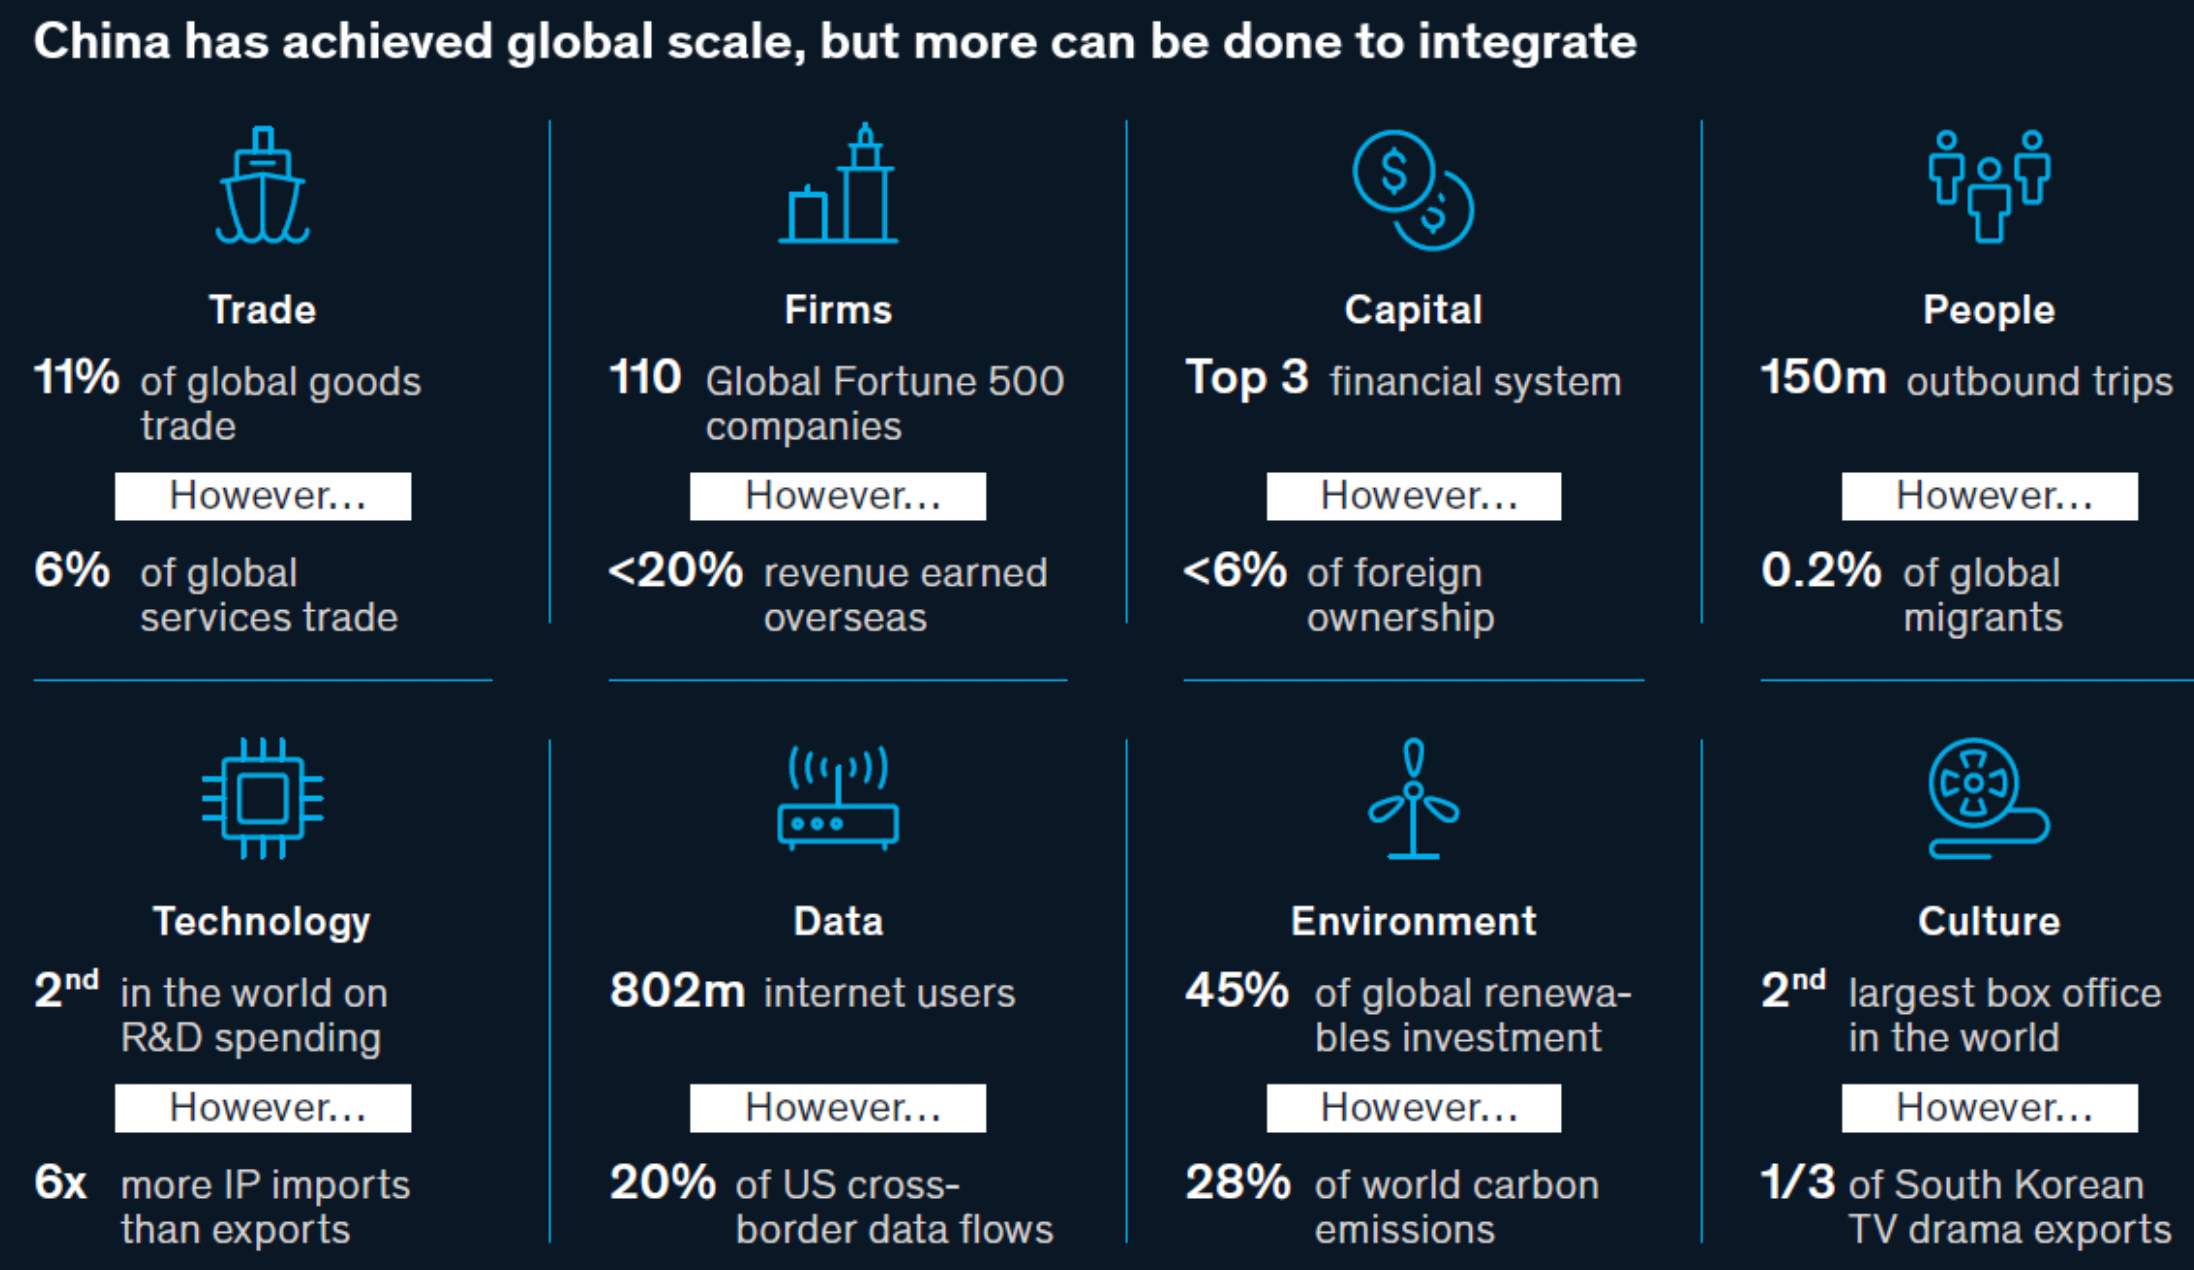
\includegraphics[width=15cm]{../images/EnpRisk_Fig11-1}
    \centering
\end{figure}

Let us take a closer look at the importans and exports between Switzerland and China.

\textbf{Swiss exports to China ($\$21.7B$):}

\begin{itemize}
    \item Gold $37.4\%$
    \item Packaged Medical Goods $9.81\%$
    \item Blood, antisera, vaccines, toxins and cultures $9.53\%$
    \item Base Metal Watches $6.79\%$
\end{itemize}

\textbf{Swiss imports from China ($\$13.1B$):}

\begin{itemize}
    \item Computers $10.2\%$
    \item Broadcasting Equipment $10\%$
    \item Office Machine Parts $3.56\%$
    \item Jewellery $2.55\%$
    \item Nitrogen Heterocyclic Compounds $2.33\%$
\end{itemize}

\textbf{Why China needs Switzerland:}

\begin{itemize}
    \item An entry point to the European market
    \item A signal to Europe and the west advanced economies
    \item An entry point to the global stage via international organizations
    \item A neutral and friendly country
    \item A balance with Europe and the US
\end{itemize}

\textbf{Why Switzerland needs China:}

\begin{itemize}
    \item A huge competitive market
    \item Engagement in an emerging power in the global stage
    \item A balance with Europe and the US
    \item A client that Switzerland has been selling its neutrality service to
\end{itemize}

\subsection{China as a Planet with different Value System}

China's culture can be named as \textbf{Confucianism.} The maind foundations of Confucianism emphasize duty, sincerity, loyalty, honor, filial piety, respect for age and seniority. As individuals maintaint harmonious relations among themselves, society itself becomes stable.

Chinese business culture is largely influenced by Confucianism:

\begin{itemize}
    \item The Confucian concept of Guanxi means that a relationship network is crucial and absed on the values of solidarity, loyalty, modesty and courtesy.
    \item Hierarchy in China, both in business and privacy, is purely vertical and highly respected.
    \item Chinese people will be careful to save face in order to protect individual reputations, influence and dignity.
\end{itemize}

\textbf{Collectivism vs. individualism} is referred to as the degree which individuals in a certain country prefer acting as individuals rather than as members of groups. This dimension focuses on the relationship between the individual and the larger social groups.

It encourages poeple to pull up their socks and get out of poverty. On the other hand, China as a collectivstic society encourages more group work and puts more emphasis on strong relationships between individuals hence the basis of guanxi. To them, the needs of a group are way more important than individual needs.

\textit{Characteristics of individualistic cultures:}

\begin{itemize}
    \item Fosters contractual relationships that revolve around the basics of exchange.
    \item Concentrates more on self and the very dear or near ones.
    \item More emphasis on personal pleasure, over dutions, fun, enjoyment and social norms.
    \item Value independence and self-sufficiency with self-interest placement.
    \item They hold unique beliefs and decisions are made based on individual needs.
\end{itemize}

\textit{Charactersitics of collectivistic cultures:}

\begin{itemize}
    \item Behavior must subscribe to the social norms established.
    \item More giving up of personal interest.
    \item Before making any major decisions, the implications to the wider collective must be considered.
    \item Be a part of few influential in-groups and inclining towards conformity.
    \item Much emphasis on hierarchy and harmony within the group.
\end{itemize}

After the stabiliztation in China's economy, there was a new economic shock. The economy looked to be improving before the lockdowns hit. The march lockdowns reversed China's economic momentum.

Property policy kept easing as lockdowns stopped sales. Property sales had improved but were headed back down. Housing market sentiment bottomed out in late 2021.

Fiscal spending will help stabilize growth. China's public spending will recover strongly in 2022 and infrastructure spending should have a decent rebound in 2022.

\subsection{Two Innovation Styles}

We consider innovation styles of Swiss Start-ups and Spin-offs in comparison to other startups:

\begin{table}[H]
    \begin{tabular}{l|l|l|}
                          & Swiss Start-ups       & Other Start-ups \\ \hline
    Innovation model      & Show Me               & Believe Me      \\ \hline
    Entrepreneur culture  & Conservative, prudent & Aggressive      \\ \hline
    Imapct                & Relatively low        & Higher          \\ \hline
    Industries            & High-tech mainly      & Comprehensive   \\ \hline
    Risk preference       & Low                   & High            \\ \hline
    Average return        & High                  & Low             \\ \hline
    Enterprise life       & Long                  & Short           \\ \hline
    5-year survival ratio & 50\% (ETH 93\%)       & \textless 10\%  \\ \hline
    \end{tabular}
\end{table}

China's spending on research and development in science and technology, surged ten-fold since 2000, while the U.S. spending grew a modes 39\% in the same time period. Innovation refers to the ability to produce new economic value through the creation or improvement of products or business services. China has advanced far beyond the mere copying of Western products or technologies and now excels at \textbf{incremental innovation} (a modification or ehancement to an existing product or service that improves its market position and increases its economic value). It still lags the US, Europe and Japan in \textbf{transformational} (something that fundamentally alters a market or an industry), science-based innovation, but with sustained policy focus and investment by its government, transformational innovation can also be expected to advance.

Advances are clear at the national level, in fields such as supercomputing, quantum communications, space, and robotics. In the private sector, advances can best be seen in monile commerce, where China currently leads the world.

\textbf{When bottom-up meets top-down: Switzerland's vs. China's strategies:}

\textbf{Switzerland:}

\begin{itemize}
    \item \textbf{Strategy Level:} The most innovative country in the world, ranked No. 1 for 11 consecutive years on the Global Innovative Index.
    \item \textbf{Asset Level:} \textit{High-quality assets:} 99\% of tech-driven enterprises are SMEs/start-ups. The 5-year survival ratio of ETH spin-offs is as high as 93\%. \textit{Limited European markets:} many choose to enter the US, while few choose China or Asia.
    \item \textbf{Capital Level:} \textit{High demand for VC capital:} many cutting edge and high-tech start-ups face funding gaps. \textit{Conservative Capital:} due to the cultural influence, the capital developement is limited by its risk preference.
\end{itemize}

\textbf{China:}

\begin{itemize}
    \item \textbf{Strategy Level:} national strategy of Mass Entrepreneurship and Innovation, which has been a new driving force for national developments.
    \item \textbf{Asset Level:} \textit{Wide market:} Cutting edge technology in Switzerland could be better transferred and commercially applied in China. \textit{High demand for high-quality assets:} China lacks the world's top quality innovative technology and enterprises.
    \item \textbf{Capital Level:} \textit{Adequate Capital:} after years of capital bubbles, capital tends to pursue high-quality projects. \textit{Sufficient risk tolerance and strong operational capacity:} the capital has strong capacity in technology transfer, packaging and operation.
\end{itemize}

\subsection{Risks and Opportunities}

\textbf{Risks:}

\begin{itemize}
    \item COVID-19 policies: cost of traveling, local operation of factories and supply-chains, etc.
    \item Geopolitics: US-China relations, sanctions, wars, etc.
    \item International reputation risk: mostly negative hadlines about China, US policymakers have created a cliamte of moral shame for doing business with China
    \item Local competitors: rise of local companies and the government stress of pursuing self-sufficiencies
    \item Local reculatory environment: against foreign companies, data protection, plattform companies, etc.
\end{itemize}

\textbf{Opportunities:}

\begin{itemize}
    \item Well-trained labor source and local support system
    \item Positive expectations on economig growth
    \item Expanding middle-class population and the unique consumption market
    \item Special opportunities in certain industries
\end{itemize}

\end{document}